\documentclass[runningheads]{llncs}
\usepackage{graphicx}
\usepackage{booktabs} % For formal tables
\usepackage{float} % To be able to use H (force to place image Here) when placing a figure
\usepackage{pifont} %Added for the number in round in text (ding)
\usepackage[normalem]{ulem} % use normalem to protect \emph
\newcommand\hl{\bgroup\markoverwith
{\textcolor{yellow}{\rule[-.5ex]{2pt}{2.5ex}}}\ULon}
\usepackage{xcolor} %style comment in algorithm2e algorithm
\usepackage[linesnumbered,boxed,vlined]{algorithm2e} %added for pseudocode
\newcommand\mycommfont[1]{\scriptsize\textcolor{darkgray}{#1}} %style comment in algorithm2e algorithm

\SetCommentSty{mycommfont} %style comment in algorithm2e algorithm
\usepackage{array,tabularx} %Added for legend in mathematical formulas
\usepackage{multirow}

\newcolumntype{L}[1]{>{\raggedright\let\newline\\\arraybackslash\hspace{0pt}}m{#1}}

\usepackage{bm}
\usepackage{amssymb} %added for right triangle
\usepackage{wrapfig} %floating img

\newenvironment{conditions*}
{\par\vspace{\abovedisplayskip}\noindent
\tabularx{\columnwidth}{>{$}l<{$} @{\ : } >{\raggedright\arraybackslash}X}}
{\endtabularx\par\vspace{\belowdisplayskip}}

\begin{document}
%
\title{Accurate and Transparent Path Prediction \\ Using Process Mining}
\titlerunning{Path Prediction Using Process Mining}
%
%\titlerunning{Abbreviated paper title}
% If the paper title is too long for the running head, you can set
% an abbreviated paper title here
%
\author{Ga{\"e}l Bernard\inst{1} \and
Periklis Andritsos\inst{2}}
%
\authorrunning{G. Bernard et P. Andritsos}
% First names are abbreviated in the running head.
% If there are more than two authors, 'et al.' is used.
%
\institute{University of Lausanne, Faculty of Business and Economics (HEC), Switzerland \email{gael.bernard@unil.ch} \and
University of Toronto, Faculty of Information, Toronto, Canada, \email{periklis.andritsos@utoronto.ca}
}
%
\maketitle 

\begin{abstract}
Anticipating the next events of an ongoing series of activities has many compelling applications in various industries. It can be used to improve customer satisfaction, to enhance operational efficiency, and to streamline health-care services, to name a few. In this work, we propose an algorithm that predicts the next events by leveraging business process models obtained using process mining techniques. Because we are using business process models to build the predictions, it allows business analysts to interpret and alter the predictions. We tested our approach with more than 30 synthetic datasets as well as 6 real datasets. The results have superior accuracy compared to using neural networks while being orders of magnitude faster.

\keywords{process mining, predictive process monitoring, predictive analytics, path prediction, trace clustering}
\end{abstract}


\section{Introduction}

After observing a few events of an incomplete sequence of activities, we can predict the next events until process completion by learning from historical event logs, an activity coined path prediction \cite{polato2018time}. Anticipating the next events is valuable in a wide range of scenarios. For instance, when a service desk team predicts the paths taken by open tickets, the results can be used in many different ways. One proposition is to cut the number of predicted complaints due to delays by changing the priority of tickets. Another is to reduce the negative impact on customer satisfaction by preemptively informing them about a delay. One more is to align the expertise of service desk agents with the events predicted for a ticket. The predictions could also be used by inexperienced agents to anticipate the next events better, allowing them to communicate more accurate information to the customers. Overall, predicting paths can help to improve worker and customer satisfaction, as well as improve operational efficiency.

There are two main approaches to making predictions for a series of events. The first uses process mining while the second relies on neural networks. Both approaches have their strengths and limitations. Process mining is more transparent because it relies on models that can be inspected by business analysts. This is important, as business analysts may have hidden knowledge that will influence their confidence in the prediction. Furthermore, ``business stakeholders are not data scientists [...] they are more likely to trust and use these models if they have a high-level understanding of the data that was used to train these models'' \cite{Gartner2018ExplainableAI}. In contrast, reasoning about predictions made by artificial neural networks is complex, if not impossible. Furthermore, a neural network requires a long training time \cite{polato2018time}. However, in terms of performance, the most recent research shows that predictions using long short-term memory (LSTM) in a neural network achieves high accuracy \cite{tax2017predictive}.

We address the research gap that exists between accurate, but black-box techniques and transparent, but less accurate process mining approaches. Indeed, we aim to make predictions that are accurate, fast, and interpretable by business analysts. We propose a matrix named the loop-aware footprint matrix (LaFM), which captures the behaviors of event logs when replayed on a business process model obtained automatically using process mining techniques. The captured behaviors are then retrieved from LaFM to make predictions about uncompleted traces. We also propose a clustered version of LaFM (c-LaFM) that can cope with the inherent complexity of real datasets. We evaluate the prediction accuracy of LaFM with 30 synthetic datasets and the accuracy of c-LaFM with 6 real datasets. We show that our technique outperforms the LSTM approach introduced in \cite{tax2017predictive}.

The paper is organized as follows. In Section 2, we introduce the main definitions and discuss process mining. Section 3 provides an overview of existing works. Section 4 presents the main idea behind LaFM. In Section 5, we present the evaluation procedure. Section 6 evaluates and compares the accuracy of the method using synthetic datasets. Section 8 introduces the clustered version of LaFM, coined c-LaFM, which is evaluated in Section 8. The paper ends in Section 9 with a conclusion.

\section{Preliminaries}
In this section, we lay out the main definitions and concepts of our approach. They are part of the well-established process mining discipline. In this paper, we consider only the sequence of events, disregarding the timestamps or any other contextual information in the data. By doing so, we present a simplified view of process mining, to be complemented with the foundational book about process mining \cite{van2016process}.

\textbf{Events.} An event is a discrete type of data representing the activities executed in a process. For instance, ‘transferring a ticket’ is an event in a ticket's lifecycle. Let $e$ be an event and $E$ be the set of all distinct events; i.e., $e \in E$. 

\textbf{Trace.} A trace is an instance of a process execution. In a service desk context, a trace is a ticket. Let $t = \{e_1, e_2, ...; e \in E \}$ be a trace: a list of events. For instance $\langle \textsc{abbc} \rangle$ is a trace with three distinct events of length 4 ($|t|=4$).

\textbf{Prefix.} Let a prefix $p_n = \{e_1, e_2, ..., e_n; e \in t\}$ be the first $n$ events of a trace. Typically, if $t = \langle \textsc{abbc} \rangle$, then $p_3 = \langle \textsc{abb} \rangle$. A prefix represents the few  events observed from an uncompleted trace that we use to make a prediction.

\textbf{Suffix.} A suffix represents the $n$ last events of a trace. Formally, $s_n = $ $\{e_{|t|-n}$ $, ..., e_{|t|-1}, e_{|t|}; e \in t; e \notin p_n; |p_n|+|s_n| = |t|\}$, i.e., the suffix is the complement of the prefix. The suffix is the set of events that we are trying to predict.

\textbf{Event logs.} An event log $L = \{t_1, t_2, ...;\}$ is a collection of traces. 

\vspace{5pt}

By looking only at the event log, process discovery techniques allow us to infer the business process model that describes well the behavior of the traces. This is a challenging task because the algorithm should be able to generalize behaviors even if only a subset of them is observed, to exclude noise and outliers, and to discover a model that is simple enough that it can be analyzed by a business analyst but also precise enough to reflect the behaviors of the event logs. Several techniques and approaches have been proposed to tackle this task. In this work, we use the inductive miner \cite{leemans2013discovering}.


\begin{wrapfigure}{r}{0.4\textwidth}
\begin{center}
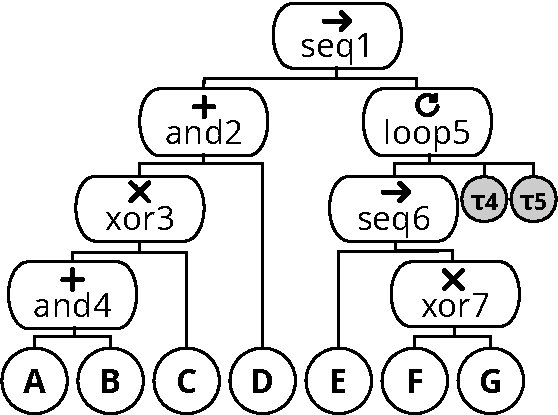
\includegraphics[width=0.35\columnwidth]{02-schema/process_tree.pdf}
\end{center}
\caption{Process tree obtained by the inductive miner with the traces: $\{ \langle \textsc{abdef} \rangle$, $\langle \textsc{bdaegef} \rangle$, $\langle \textsc{\textsc{dcefeg}} \rangle$, $\langle \textsc{cdeg} \rangle \}$.}
%\vspace{-15pt}
\label{process_tree}
\end{wrapfigure}

The inductive miner works by finding the best split in an event log and seeing how the two parts are related. It does this recursively on both parts. The output is a process tree (Fig. \ref{process_tree}), which is a representation of a process model that was introduced in \cite{vanhatalo2008refined}. A process tree uses four operators: (1) the exclusive choice operator, $\texttt{xor}$, expresses that only one of the branches is executed; (2) the parallel operator, $\texttt{and}$, indicates that all the branches should be executed, in any order; and (3) a sequence, $\texttt{seq}$, forces the execution of the branches from left to right. Finally, (4) a $\texttt{loop}$ has a more complex execution scheme: the first branch is executed at least once. Then, either we enter the loop by executing the second branch and the first branch again (which can be done once or multiple times), or we execute the third branch to exit the loop. As can be seen in Fig. \ref{process_tree}, except for the leaves, these four operators fill the whole tree. The leaves of the tree are composed of the events $E$ as well as silent activities. Silent activities, $\tau$, can be executed like any other events in the model, but they will not be seen in the traces.

We have now introduced the main terminology, the inductive miner, and the process tree. Path prediction is concerned with predicting the suffix for a given prefix by learning from event logs. It differs from process model discovery in which the goal is to discover a process model from event logs. While the output is different, both methods are about understanding the control flow of traces. We leverage this by using the inductive miner as a first step in making predictions.


\section{Related Work}

The area of predictive analytics is wide as trace predictions can be time-related (e.g., predicting the remaining time), outcome-oriented (e.g., success vs. failure), or control-flow oriented (e.g., next event(s) prediction). In this work, we specifically focus on the latter type of prediction. 

A widely adopted approach to prediction is to build a Markov chain that describes the transition probabilities between events. These transition probabilities are used to make predictions. A prediction depends only on the previously observed event. In the all-K-order Markov model, \cite{pitkow1999mininglongestrepeatin}, the number of levels in the Markov chain is increased, but this increases the execution time. While the accuracy of the prediction increases, it suffers from rigidness in terms of the ``patterns that it can learn'' \cite{gueniche2013cpt}. As another approach, Gueniche et al, propose the compact prediction tree \cite{gueniche2013cpt}. It uses three data structures that can be used efficiently to retrieve the most probable event that might occur after having observed a prefix. While it predicts with high accuracy which events might occur in the suffix, it does not return the order in which they will be executed. Hence, compact prediction trees are not suitable for predicting paths.

There are several process mining approaches for predicting paths. In \cite{lakshmanan2015markov}, Lakshmanan et al. propose a method that estimate the likelihood of the next activities using a process model and Markov chain. Breuker et al. propose in \cite{breuker2016comprehensible} a predictive framework that uses grammatical inference and an expectation-maximization algorithm to estimate the model parameters. Among its predictions, it can predict the next event. Improving the comprehensibility of the predictions is one of the design goals of their approach, so that ``users without deep technical knowledge can interpret and understand'' \cite{breuker2016comprehensible}. In \cite{polato2018time}, Polato et al. propose a labeled transition system and methods for several predictive analytic tasks. Path prediction can be done by finding a path in the transition system that minimizes the sum of the weights between the edges.

Recently, neural networks have been studied for predicting the next events. To the best of our knowledge, Evermann et al. were the first to use a LSTM neural network approach to predict the next event of an ongoing trace \cite{evermann2016deep}. LSTM, \cite{hochreiter1997long}, is a special type of neural network for sequential inputs. It can learn from long-term dependencies using a sophisticated memory system. The sophisticated memory system is a double-edged sword: it achieves high accuracy; however, its inherent complexity prevents any inspection of the reasoning behind the predictions. In \cite{tax2017predictive}, Tax et al. generalize the approach of \cite{evermann2016deep}. They evaluate--amongst other methods--the performance of the algorithm in path prediction and show that it is more accurate than \cite{evermann2016deep,breuker2016comprehensible,polato2018time}. Because it achieves the best accuracy, we use it as a baseline when evaluating the accuracy of LaFM.

Overall, two streams of research dominate path prediction. On one hand, using process mining techniques, we can make predictions using models that can be inspected by business analysts. On the other hand, neural networks attain better performance in terms of accuracy. Our contribution is an algorithm that utilizes the best aspects of both methods.


\section{LaFM: Loop-Aware Footprint Matrix}
\label{Section:LaFM}
We designed LaFM to store the behavior of traces efficiently when replayed on business process models. The aim is that the behaviors can be retrieved when predicting a suffix of events. First, we present the LaFM data structure. Next, we explain how to build it. Finally, we detail how to use it to make predictions.


\subsection{LaFM Data Structure}
LaFM records the behavior of traces when replayed on top of a business process model. An illustration of LaFM is shown in Fig. \ref{LaFM}. Each row corresponds to a trace and each column describes the behavior of an operator. LaFM captures the execution orders of parallel branches, the exclusive choices, and the number of iterations of each loop. We next describe in more detail the information recorded by LaFM as well as the used terminology.

\begin{figure}[H]
\begin{center}
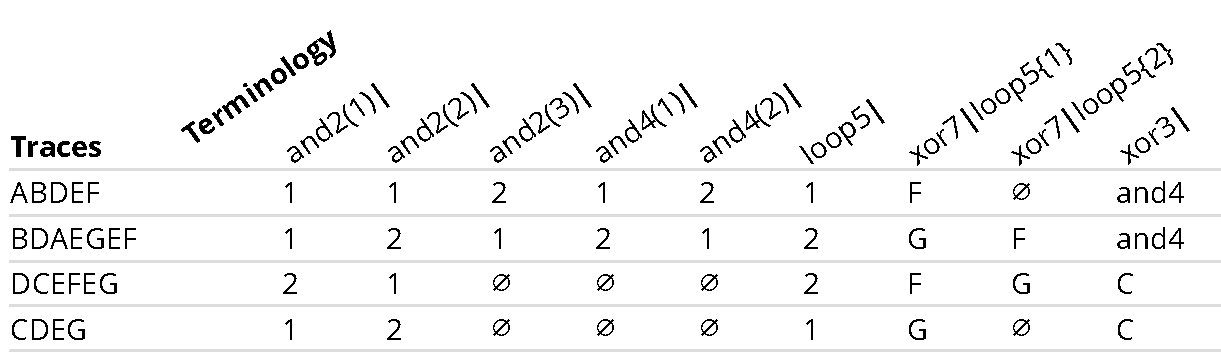
\includegraphics[width=1\columnwidth]{02-schema/LaFM.pdf}
\caption{Result of LaFM when the traces $\langle \textsc{abdef} \rangle$, $\langle \textsc{bdaegef} \rangle$, $\langle \textsc{dcefeg} \rangle$, and $\langle \textsc{cdeg} \rangle$ are replayed on top of the process tree of Fig. \ref{process_tree}. }
\label{LaFM}
\end{center}
\end{figure}


\subsubsection{Parallel branches.} LaFM stores the order in which parallel branches are executed. An incremental index is assigned to each outgoing branch of the $\texttt{and}$ operators and then propagated to the events and silent activities underneath. For instance, $\texttt{and2}$ in Fig. \ref{process_tree} has two outgoing branches. The index 1 is assigned to the first branch, which is propagated to the events below, i.e., 1 is assigned to $\textsc{a}$, $\textsc{b}$, and $\textsc{c}$. Similarly, task $\textsc{d}$ has index 2. The index is recorded in LaFM for each $\texttt{and}$ operator


\subsubsection{Exclusive choices.} The decision made for each exclusive choice is recorded in LaFM. For example, at $\texttt{xor3}$ in Fig. \ref{process_tree}, a choice must be made between $\texttt{and4}$ and $\textsc{c}$. For the trace $\langle \textsc{cdeg} \rangle$, the choice is $\textsc{c}$. Hence, $\textsc{c}$ is recorded in LaFM.

\subsubsection{Loops.} LaFM stores the number of times loops are executed. In Fig. \ref{process_tree} for the trace $\langle \textsc{cdeg} \rangle$, the value recorded for $\texttt{loop5}$ is $1$ because it was executed once.


\subsubsection{Terminology.}
An operator might be executed multiple times during a single process execution. For instance, when the trace $\langle \textsc{bdaegef} \rangle$ is replayed on the process tree in Fig. \ref{process_tree}, we execute the operator $\texttt{xor7}$ twice because $\texttt{loop5}$ above it is also executed twice. The name ‘loop-aware footprint matrix reflects that the matrix can store all behaviors, regardless of the number of times a loop is executed. The terminology used for columns in LaFM allows us to retrieve the behaviors of an operator using a standardized name: {$\texttt{operator\textbf{\textbar}loop}$}. Each operator is assigned a unique name. For example, in Fig. \ref{process_tree}, $\texttt{loop5}$ is an operator. For parallel gateways, we also append the execution order inside parentheses. For instance, the second execution of $\texttt{and4}$ is $\texttt{and4(2)}$. If there are loops, a single operator can be executed many times, resulting in multiple pieces of information that must be recorded. Adding the loop position to the terminology allows us to distinguish this information. Let $L$ be a list of loops that are in the path starting from but excluding the operator itself to the root of the process tree. $L$ can be empty if an operator is not contained in a loop. Then, we concatenate $\forall l \in L$ the following strings: $l_{name}(l_{index})$, i.e., for each loop above an operator, we include its name. In parentheses, we add the index of the loop. As an example, $\texttt{xor7|loop5\{2\}}$ points to the column returning the decisions that are made when the operator $\texttt{xor7}$ is executed for the second time.

Three behaviors are captured in the LaFM in Fig. \ref{LaFM}. Columns 1 to 5 retain the execution order of parallel gateways; column 6 records the number of times a loop was taken, and columns 7 to 9 store the decisions made at exclusive choice gateways. 

\subsection{Training phase: building LaFM} \label{Section:buildingPhase}
To record the decisions made for each operator in the discovered process tree, we replay the traces we want to learn from a Petri net version of the process tree. Petri nets can easily be derived from process trees using simple transformation rules \cite{leemans2013discovering}. Petri nets have a strong and executable formalism, which means we can replay a trace on a Petri net by playing the token game \cite{leemans2017robust}. The token game takes as input a trace and a Petri net. Then, using a particular set of rules (see Chapter `3.2.2 Petri Nets' in \cite{van2016process}), the game indicates if the trace fits into the process model (i.e., the Petri net). Algorithm \ref{alg:recording} defines few extra operations that are performed during the token game to build LaFM. The next section explains how predictions can be made from LaFM.


\begin{algorithm}[H]
\scriptsize
\SetKwProg{Fn}{function}{:}{}

\label{alg:recording}

\tcc{Map the parallel operators above the events using a list of tuples (andOperator, branchIndex). Return an empty list if the event is not included in a parallel operators.}
\tcc{ e.g.,: \{a: [(and4,0), (and2,0)], b: [(and4,1), (and2,0)], c: [(and2,0)]...\} }
tsToAnds = getTransitionToAnds($processTree$) \\ 
\vspace{0.4em}
\tcc{Map the transitions that occur right after an exclusive gateway.}
\tcc{ e.g.,: \{$\texttt{and4}$: Xor3, $\textsc{c}$: Xor3, $\textsc{f}$: Xor7, $\textsc{g}$: Xor7 \} }
tsToXors = getTransitionToXor($processTree$) \\
\vspace{0.4em}
\tcc{ Map the second branch of loops to tsIncrementLoops and the third one to tsLeavingLoops}
\tcc{ e.g., tsIncrementLoops: \{$\tau4$: loop5\}; tsLeavingLoops: \{$\tau5$: loop5\} }
tsIncrementLoops = getTransitionToIncrementLoop($processTree$) \\
tsLeavingLoops = getTsToLeaveLoop($processTree$) \\
\vspace{0.4em}
laFM = Matrix[] \\

\end{algorithm}

\begin{algorithm}[H]

\setcounter{AlgoLine}{5}
\scriptsize
\SetKwProg{Fn}{function}{:}{}


\ForEach{$trace$ in $logs$}{
counter = initializeCounters() \\
\ForEach{$tsFired$ in $tokenGame$}{
manageCounter($tsFired$) 

\ForEach{$andOperators$ in $tsToAnds[tsFired]$}{
\ForEach{$andOperator, branchIndex$ in $andOperators$}{
record($trace$, $andOperator$, $branchIndex$)
}
}
\If{$tsFired$ in $tsToXors$}{
record($trace$, $tsToAnds[tsFired]$, $tsFired$)
}
\If{$tsFired$ in $tsToLeaveLoop$}{
record($trace$, $tsLeavingLoops[tsFired]$, $counter[tsFired]$)
}
}
}

\Fn{manageCounter($tsFired$)}{
\If{$tsFired$ in $tsToAnds$}{
\ForEach{$andOperator$ in $tsToAnds[tsFired]$}{
counter[$andOperator$].increment()
}
}
\If{$tsFired$ in $tsIncrementLoops$}{
counter[$tsFired$].increment()

\ForEach{$dependentTransition$ in $dependentTransitions[tsFired]$}{
counter[$tsFired$].reset()
}
}
}

\Fn{record($trace$, $transition$, $value$)}{
laFM[$trace$][getTerminology($transition$)] = $value$
}



\caption{Set of extra operations performed during the token game to build LaFM.}
\end{algorithm}

\subsection{Prediction Phase: using LaFM} \label{Section:predictionPhase}

Making predictions using LaFM is a five step recursive process, illustrated in Fig. \ref{fig:predictionAbstract}.  

\begin{figure}
\begin{center}
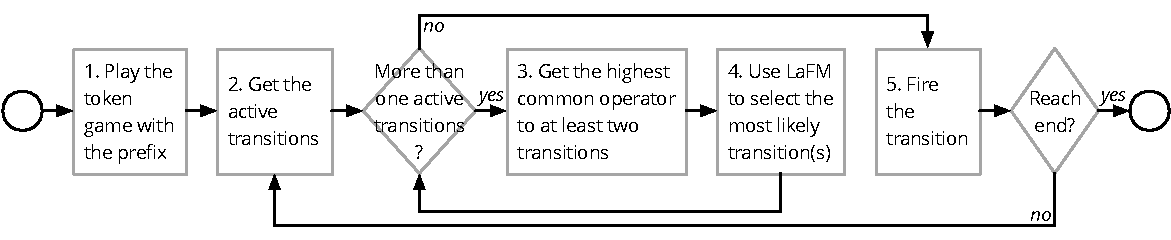
\includegraphics[width=1\columnwidth]{02-schema/predictionAbstract.pdf}
\caption{Five steps in making prediction using LaFM}
\label{fig:predictionAbstract}
\end{center}
\end{figure} 


\subsubsection{Step 1.} We play the token game with the prefix to get a list of active tokens. 

\subsubsection{Step 2.} From the tokens, we get the list of active transitions, i.e., the activities that are currently allowed by the business process model. If only one transition is active, we skip steps 3 and 4 to fire the transition (step 5). Otherwise, we recursively eliminate transitions that are less likely (steps 3 and 4). 

\subsubsection{Step 3.} We find the highest (closest to the root) operator in the process tree common to at least two transitions. For example, in Fig. \ref{process_tree}, if the active transitions are $\textsc{a}$, $\textsc{b}$, and $\textsc{d}$, the highest common operator is $\texttt{and2}$.


\subsubsection{Step 4.} We make a decision about the operator selected in step 3. Depending on the operator type, we select the branch to execute next, what decision to make at an exclusive gateway, or whether to stay in or leave a loop. Fig. \ref{fig:decision} details how we retrieve the information in LaFM. In Fig. \ref{LaFM}, in order to know which one of $\textsc{f}$ and $\textsc{g}$ is the transition most likely to be chosen the first time we are at $\texttt{xor7}$, we look at LaFM for $\texttt{xor7|loop5\{1\}}$ and observe that $\textsc{f}$ occurs more often (three times out of four). When a tie occurs, we pick the first one. The number of loops in the prefix might exceed the number of loops that were observed in the data. Alternatively, we might have a particular order in the prefix that was never observed in the event logs. We define three levels of abstraction that we apply consecutively when the previous abstraction fails. The first level of abstraction is to use LaFM as is. The second level of abstraction is to drop the loop part of the terminology and stack the columns for the same operator. For example, if $\texttt{xor7|loop5\{3\}}$ does not exist in LaFM, we stack the two columns starting with $\texttt{xor7|}$. If there is still not enough information, the third abstraction is to make a decision by looking only at the Petri net. For parallel and exclusive choice transitions, we pick the first branches with active transitions. For a loop, the decision is to always to leave the loop. Using these three abstractions, we can always make a prediction. If the list of potential transitions has been reduced to 1, we go to step 5. Otherwise, we recursively go back to step 3 where the highest common operator will inevitably be lower.
 
\begin{figure}
\begin{center}
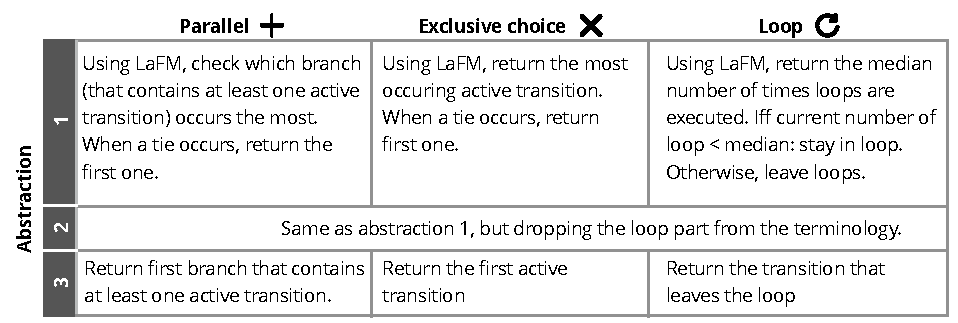
\includegraphics[width=1\columnwidth]{02-schema/decision.pdf}
\caption{Decisions for each operator type at three level of abstractions.}
\label{fig:decision}
\end{center}
\vspace{-10pt}
\end{figure} 


\subsubsection{Step 5.} We fire the transition. If it is a task $\in E$, we add it to the suffix. Then, we check to see if we have reached the end of the Petri net. If yes, we return the suffix. If not, we go back to step 3.

% The table \ref{table:predictionType} provides an overview of the decisions that can be retrieved for each operator type.

% \begin{figure}[t]
% \begin{center}
% 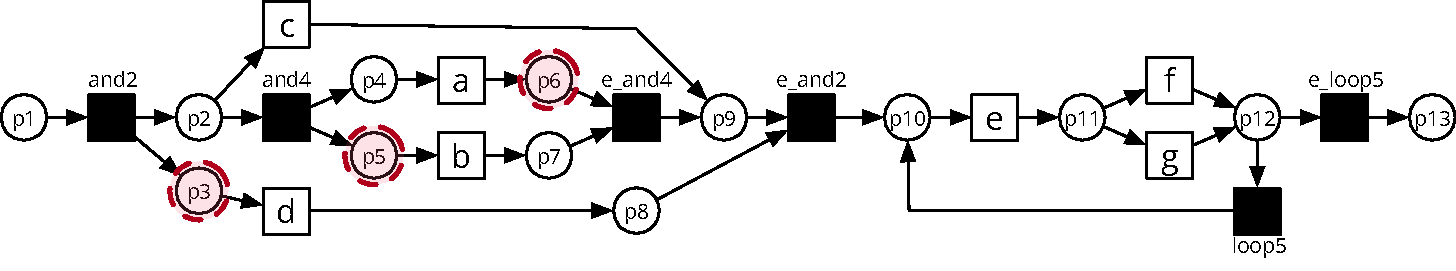
\includegraphics[width=1\columnwidth]{02-schema/petri_net.pdf}
% \label{fig:petri_net}
% \caption{Petri Net derived from the process tree visible in Fig. \ref{process_tree}. The three red circle symbolize the tokens positions after replaying the prefix $\langle a \rangle$}
% \end{center}
% \end{figure} 

% \begin{algorithm}[H]
% \scriptsize
% \SetKwProg{Fn}{function}{:}{}

% \label{alg:replaying}

% $suffix$ = getSuffix($prefix$) \\

% \Fn{getSuffix($prefix$)}{ 

% 	$activeTransitions$ = replayPrefix($prefix$) \label{algorithm:lineactiveTransitions} \\
% 	$suffix$ = $\emptyset$ \\

% 	\While{not reachingEndOfPetriNet()}{

% 		\tcc{ Get the highest operator (i.e., closest to root) in the process tree which is common to at least two active transactions}
% 		$operator$ = GetHighestCommonOperator($processTree$, $activeTransitions$) \label{algorithm:GetHighestCommonOperator} \\
% 		$nomenclature$ = GetNomenclature($operator$) \\

% 		$nextTransition$ = chooseNextTransitionToFire($nomenclature$, $laFM$) \label{algorithm:chooseNextTransitionToFire} \\
% 		$activeTransitions$ = fire($nextTransition$) \\
% 		\If{$nextTransition$.type is 'task'} 
% 		{$suffix$.add($nextTransition$)} \label{appendToSuffix}
% 		return $suffix$
% 	}
% }

% \Fn{chooseNextTransitionToFire($nomenclature$, $laFM$)}{ \label{chooseNextTransitionToFire}
    
%     \If{getTransitionType($nomenclature$) is \textsf{'}loop\textsf{'}}{
%     	$method$ = \textsf{'}median\textsf{'}
%     }
%     \Else{
%     	$method$ = \textsf{'}mode\textsf{'}
%     }

% 	\tcc{METHOD 1: Using LaFM.}
% 	$value$ = getValue($LaFM$, method=$method$, excludeEmptySet=True) \label{abstraction1}

% 	\tcc{METHOD 2: Using abstracted LaFM (i.e., dropping loop part of nomenclature).}
% 	\If{$value$ is $\emptyset$} {
% 		$value$ = getValue($abstractedLaFM$, method=$method$, excludeEmptySet=True) \label{abstraction2}
% 	}

% 	\tcc{METHOD 3: Not using LaFM.}
% 	\If{$value$ is $\emptyset$} {
% 		\If{getTransitionType($nomenclature$) is \textsf{'}loop\textsf{'}}{
% 			$value$ = getTransitionLeavingLoops($processTree$) \label{abstraction3-loop}
% 		}
% 		\Else{
% 			$value$ = getFirstActiveTransaction($processTree$)\label{abstraction3-and-xor}
% 		}
% 	}

% 	return $value$

% }

% \caption{Mechanism to make predictions using LaFM.}
% \end{algorithm}



Having defined how to build and use LaFM, we detail in the next section the evaluation procedure used to assess the quality of the predictions.

% \begin{table}[]
% \caption{Types of prediction per operator}

% \label{table:predictionType}
% \scriptsize

% \begin{tabular}{|p{1.2cm}|p{4.2cm}|p{3.6cm}|p{2.2cm}|p{0cm}}
% \cline{1-4}
% & First attempt: & Second attempt: & Last attempt: & \\ 
% & nomenclature: \textbf{operator$\vert$loop} & nomenclature: \textbf{operator$\vert$} & without LaFM & \\ \cline{1-4}
% and & Using the nomenclature, get the most occurring branch in LaFM (which contain at least one active transition) & \multirow{3}{3cm}{Same as first attempt but dropping the loop from the nomenclature} & \multirow{2}{1.5cm}{Select the first branch containing an active transition} & \\ \cline{1-2}
% exclusive choice & Using the nomenclature, return the most occurring choice (which is still active) & & & \\ \cline{1-2} \cline{4-4}
% loop & Using the nomenclature, get the median. Iff median\textbackslash{}textgreater current, stay in loop. Otherwise leave the loop & & Leave the loop & \\ \cline{1-4}
% \end{tabular}
% \end{table}

\section{Evaluation Procedure} \label{section:evalationProcedure}
The evaluation procedure is the same as that described by Tax et al. in \cite{tax2017predictive}. Two-thirds of the traces in the event logs are added to the training set. Each trace in the evaluation is tested from a prefix length of 2 to a prefix length of $l - 1$, $l$ being the length of the trace. For instance, the trace $\langle \textsc{abcd} \rangle$ is decomposed into: prefix:$\langle \textsc{ab} \rangle$, suffix:$\langle \textsc{cd} \rangle$ and prefix:$\langle \textsc{abc} \rangle$, suffix:$\langle \textsc{d} \rangle$. The extracted prefix is added to the evaluation set and the suffix is added to the ground truth set. After learning from the training set, we use the evaluation set to make predictions about the prefix. The accuracy is obtained by measuring the Damerau-Levenshtein similarity between the predicted suffix and the ground truth set. The Damerau-Levenshtein distance, \cite{damerau1964technique}, is an edit-distance-based metric that minimizes the number of substitutions, deletions, or additions that are needed to align two sequences. In contrast with the Levenshtein distance, the Damerau-Levenshtein distance allows us to swap two adjacent activities. Let $e$ be the evaluation set, $p_i$ the i\textsuperscript{th} predicted suffix, and $t_i$ the i\textsuperscript{th} ground truth suffix. We evaluate a whole evaluation set using the following formula:

\begin{equation}
	DamerauSimilarity(e) = 1- \frac{\sum_{i=1}^{|e|}{\frac{DamerauDistance(p_i,t_i)}{max(length(p_i),length(t_i))}}}{|e|}
\end{equation}

A Damerau similarity of 1 means that the predicted suffix is identical to the ground truth. We use the evaluation procedure in the next section to evaluate the performance of LaFM on synthetic datasets as well as in Section \ref{section:c-LaFM:evaluation} where the performance of c-LaFM is tested on real datasets. 

All evaluations were processed on a Mac Pro with the following configuration: 3.5 GHz 6-Core Intel Xeon E5, 64 GB 1866 MHz DDR3. We slightly updated LSTM\footnote{available here: https://verenich.github.io/ProcessSequencePrediction/} so that it does not predict the time remaining. We confirmed that this change does not impact the accuracy of the next event predictions and slightly reduces the execution time. LaFM and c-LaFM, as used in the evaluations, are available at: \url{http://customer-journey.unil.ch/lafm}


\section{LaFM: Evaluation} \label{section:laFM_evaluation}
To evaluate LaFM, we used a collection of 30 synthetic datasets\footnote{https://data.4tu.nl/repository/uuid:745584e7-8cc0-45b8-8a89-93e9c9dfab05, sets `1 - scalability', `round 3 to 5'} that were created from process trees of varying shapes and complexities. These datasets were initially created and used in \cite{leemans2017robust} for testing process discovery and conformance checking techniques. 

There are three rounds of evaluation. In each round, 10 process trees were generated. The complexity of the process trees as well as the number of traces generated increase with the round. Overall, 64 traces were generated in round 3, 256 traces in round 4, and 1025 in round 5. We compared the predictions obtained using LaFM, Markov chains, and LSTM. We ran the evaluation five times. The arithmetic means of these five runs is shown in Fig. \ref{results_synthetic}. LaFM is deterministic, therefore, its variance is null. The predictions made using LaFM are closest to the ground truth (21 times), followed by LSTM (8 times), and Markov chains (4 times). 

There are important differences in the execution times of the three techniques (Fig. \ref{fig:time_synthetic}). Because its predictions rely only on the previous observed event, it is not surprising that the fastest predictions are made using Markov chains, followed by LaFM. To put the duration into perspective, the average execution time per dataset is approximately 111 times slower for LaFM compared to a Markov chain, and 6140 times slower for LSTM compared to a Markov chain.


\begin{figure}[H]
\begin{center}
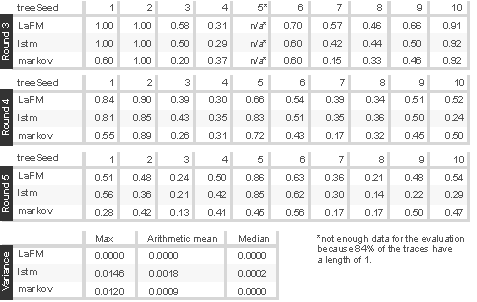
\includegraphics[width=.95\columnwidth]{02-schema/results_synthetic.pdf}
\caption{Comparing LaFM, LSTM and Markov Chains using the Damerau similarity metric. The closer to 1, the closer the predictions are to the ground truth.}
\label{results_synthetic}
\end{center}
\vspace{-20pt}
\end{figure}

\begin{figure}
\begin{center}
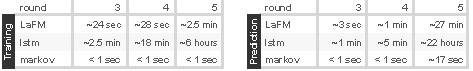
\includegraphics[width=.95\columnwidth]{02-schema/time_synthetic.pdf}
\caption{Performance comparison of the training and predictions times.}
\label{fig:time_synthetic}
\end{center}
\vspace{-20pt}

\end{figure}


\section{c-LaFM: Clustered Loop-Aware Footprint Matrix}

The accuracy of the predictions made using LaFM is dependent on the quality of the discovered process tree. While the previous section showed that LaFM performs well with synthetic datasets generated from well-structured process trees, the accuracy will drop with real datasets, which often have very complex behaviors and noise that cannot be described well using a single model. Our intuition is that we should group similar traces using clustering techniques and, for each group, discover a process tree that well describes a subset of similar traces. Hence, we propose an updated version of LaFM with a clustering step, coined c-LaFM for clustered LaFM.


\begin{figure}
\begin{center}
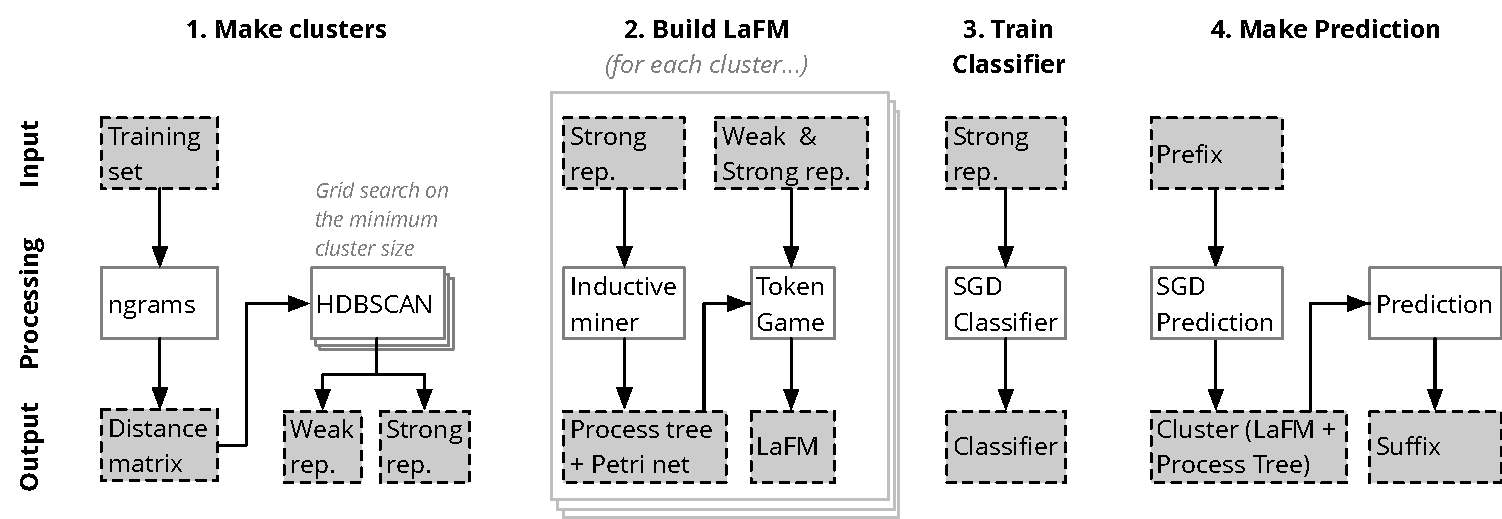
\includegraphics[width=1\columnwidth]{02-schema/LaFM_details.pdf}
\label{fig:LaFM_details}
\caption{Overview of the 4 steps approach of c-LaFM.}
\end{center}
\end{figure}

We propose a four-step clustering method, as shown in Fig. \ref{fig:LaFM_details}. In step 1, we extract the features that will be used to group similar traces. Thus, we count the number of ngrams ranging in size from 1 to 2. For instance, the trace $\langle \textsc{aba} \rangle$ becomes: \{$\textsc{a}$:2, $\textsc{b}$:1, $\textsc{ab}$:1, $\textsc{ba}$:1\}. Then, we cluster the traces using HDBSCAN\footnote{https://github.com/scikit-learn-contrib/hdbscan}, which has the advantage of having only one intelligible parameter to set, the minimum number of traces per cluster. According to our experiment, from 2 to 10 traces per cluster yields the best results. However, it is difficult to anticipate the best minimum cluster size. Hence, we perform a hyperparameter optimization of a type grid search by using 10\% of the training data set to evaluate the accuracy of the minimum cluster size and retain the best-performing one. Instead of attributing each trace to a single cluster, we rely on a soft clustering approach, which returns, for each trace, the probability of it belonging to all the clusters. 



Fig. \ref{fig:soft_clustering} illustrates the soft clustering approach. Each point represents a trace. The closer two traces are, the more ngrams they share. The strong representatives are used to discover the process tree, while the weak and the strong representatives will be replayed over the process tree and are available in LaFM. The strong representatives are the traces that have a probability higher than 80\% of belonging to a cluster and the weak representatives have a probability higher than 20\% but less than 80\%. Using a soft clustering approach has two main advantages. First, the inductive miner is sensitive to noise. Hence, we want to learn only from the strong representatives (i.e., with a high probability of belonging to the clusters) with the aim of capturing only the core behaviors. Second, although we do not use them to build the process trees, borderline traces might contain interesting behaviors for several clusters. By using a soft clustering approach, we can assign these single traces to several clusters.

\begin{wrapfigure}{l}{0.45\textwidth}
\begin{center}
\vspace{-20pt}
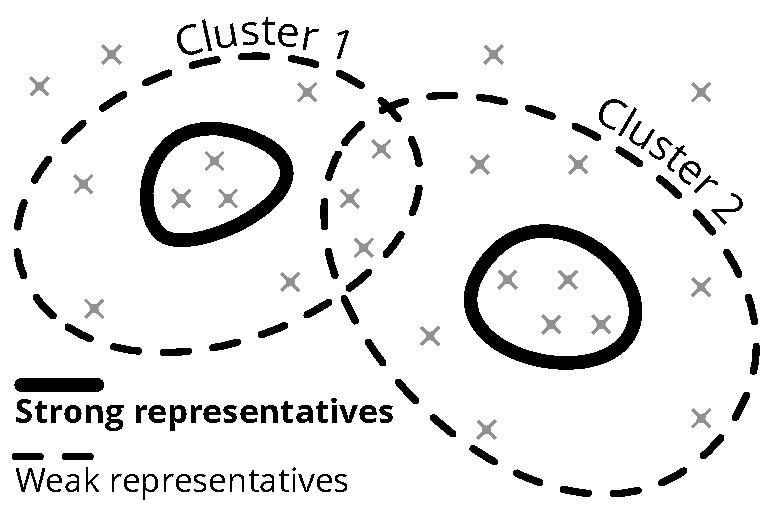
\includegraphics[width=.40\columnwidth]{02-schema/BPMN-cFM.pdf}
\end{center}
\vspace{-15pt}
\caption{Illustration of the soft clustering concept. }
\vspace{-10pt}
\label{fig:soft_clustering}
\end{wrapfigure}

In step 2, the strong representatives are used to build the process tree. Then, the process tree is transformed to a Petri net so that the weak representatives can be replayed on it to build a local LaFM, a mechanism that is described in Section \ref{Section:buildingPhase}. 

In step 3, we train a stochastic gradient descent classifier\footnote{http://scikit-learn.org/stable/modules/sgd.html} to predict which cluster a prefix belongs to. Although the clustering is done only once for the entire complete traces, we build one classifier for each prefix length. If an unexpected prefix length comes from a never-seen-before instance, we select the classifier that was built with the largest prefix length.

In step 4, we predict the suffix of a given prefix using the cluster returned by the classifier. Altogether, these four steps allow us to make predictions in the presence of noise and outliers, which are often found in real datasets. This is what we evaluate in the next section.


\section{c-LaFM: Evaluation}
\label{section:c-LaFM:evaluation}
To test our approach, we used six publicly available event logs, as described in Table \ref{table:datasets}. Because the event logs reflect activities performed in real life, making predictions is a complex task. Typically, for the event logs describing the execution of a building permit application (envPermit), ``almost every case follows a unique path'' \cite{tax2017predictive}.


\begin{table}
	\begin{center}
	\bgroup
	\def\arraystretch{1.3}
	\scriptsize
	    \begin{tabular}{ | p{0.2cm} | p{4.4cm} | p{5.2cm} | p{0.8cm} | p{1cm} | }
	    \hline
	     & Name (doi) & Description & \#traces & \#events \\
	     \hline
1 & helpdesk (10.17632/39bp3vv62t.1) & Events from a ticketing system & 3'804 & 13'710 \\
2 & bpi12 (10.4121/uuid:3926db30-f712-4394-aebc-75976070e91f) & Loan process for a financial industry. Note: keeping only manual task and lifecycle: complete as described in \cite{tax2017predictive} & 9'658 & 72'413  \\
3 & bpi13 closeP (10.4121/c2c3b154-ab26-4b31-a0e8-8f2350ddac11) & Closed problem - management system from Volvo IT Belgium & 6'660 & 1'487  \\
4 & bpi13 incidents (10.4121/3537c19d-6c64-4b1d-815d-915ab0e479da) & Incidents - management system from Volvo IT Belgium & 7'554 &  65'533  \\
5 & bpi13 openP (10.4121/500573e6-accc-4b0c-9576-aa5468b10cee) & Open problems - management system from Volvo IT Belgium & 819 & 2'351  \\
6 & envPermit (10.4121/uuid:26aba40d-8b2d-435b-b5af-6d4bfbd7a270) & Execution of a building permit application process. Note: we pick the Municipality 1 & 38'944 & 937 \\
	    \hline
	    \end{tabular}
	\egroup
\caption{Datasets used for the evaluation.}
	\label{table:datasets}

	\end{center}
	\vspace{-20pt}
\end{table}

In contrast to LaFM, c-LaFM is non-deterministic due to the clustering step. Hence, we ran the experiment 10 times with c-LaFM and LSTM using the procedure described in Section \ref{section:evalationProcedure}. Fig. \ref{c-LaFM} compares the accuracy of LSTM and c-LaFM. c-LaFM is more accurate for five datasets out of six. We compare the execution times in Fig. \ref{time_real}. On average, c-LaFM is 9 times faster than LSTM. Overall, we have shown that the clustered version of LaFM is accurate and fast.

\begin{figure}
\begin{center}
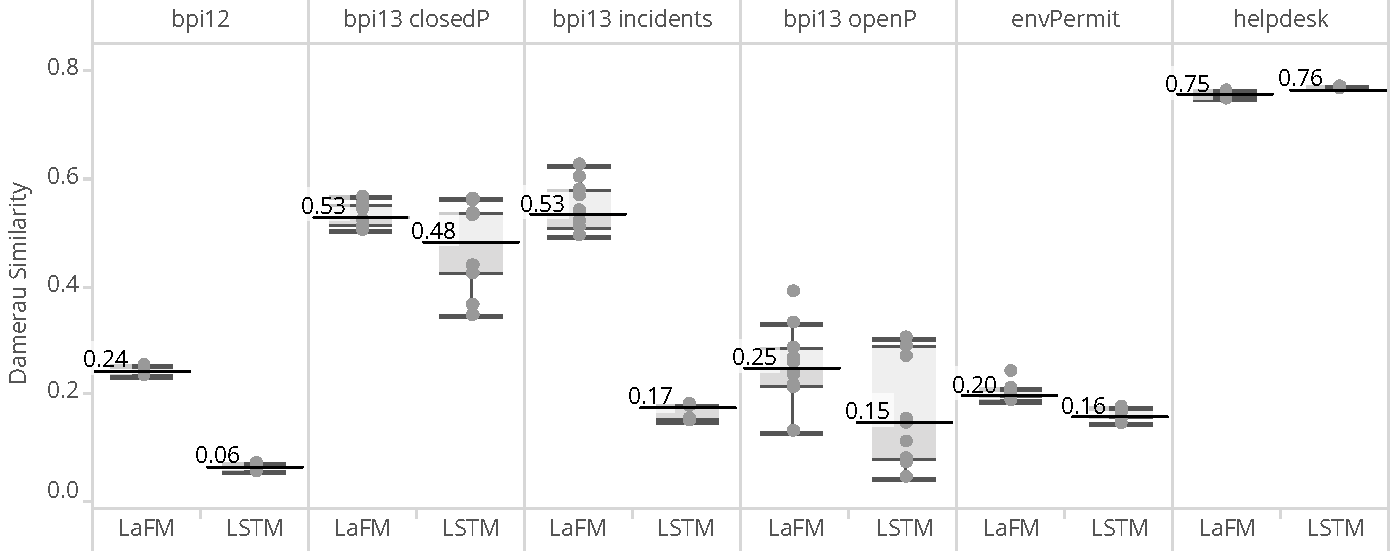
\includegraphics[width=1\columnwidth]{02-schema/results_real.pdf}
\caption{Comparing c-LaFM to LSTM using real datasets. Each datasets was evaluated 10 times. }
\label{c-LaFM}
\end{center}
\vspace{-20pt}
\end{figure}

\begin{figure}
\begin{center}
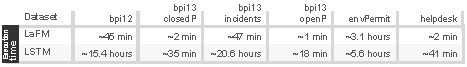
\includegraphics[width=1\columnwidth]{02-schema/time_real.pdf}
\caption{Comparing the total execution time to obtain predictions using c-LaFM and LSTM. The value reported is the average of 10 executions.}
\label{time_real}
\end{center}
\vspace{-20pt}
\end{figure}

\begin{figure}[H]
\begin{center}
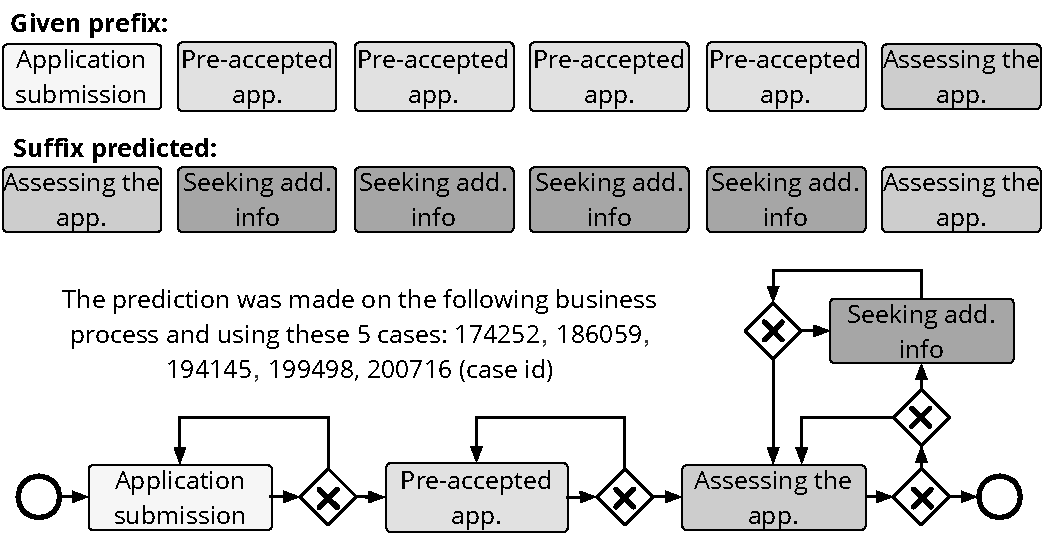
\includegraphics[width=.8\columnwidth]{02-schema/illustration.pdf}
\caption{Displaying an actual prediction from the dataset envPermit next to the business process model that was used to make the prediction. The labels has been translated in English.}
\label{fig:illustration}
\end{center}
\vspace{-10pt}
\end{figure}

Fig. \ref{fig:illustration} shows one of the predictions for the execution of a building permit using a business process model, which was derived from the process tree that was used to make the prediction. This is an illustration of how we can provide, not only the predictions itself, but a way to express the reasoning behind the prediction. For instance, a business worker could--after investigating traces like those used to make the prediction--decide not to trust the prediction because they have knowledge about the context that is not available in the event logs.

\section{Conclusion}
We propose an algorithm that relies on process models to make future path prediction. More specifically, we propose a matrix coined LaFM that retrieves the most likely next events. We also propose c-LaFM, a version which is more suited to deal with the inherent complexity of real datasets. The algorithm shows promising results in terms of accuracy and execution time. 

The results showcase the value of the process models discovered using a process discovery algorithm. Indeed, not only are these business models intrinsically interesting for business process analysts, but we also show that they can be used to make predictions. A limitation of this work is that we choose to rely on the inductive miner. In our future work, we plan to measure how the use of different process discovery techniques may impact the accuracy of the predictions. We anticipate that mining hidden rules between LaFM columns will yield interesting results, especially if we consider extending LaFM with contextual information. This would allow us to detect long-term dependencies that could be used to improve the accuracy further.

Business analysts can be reluctant to trust predictions they do not understand \cite{breuker2016comprehensible}. Because in our work the predictions are made with business process models, the predictions can be manually inspected by business analysts. Currently, our algorithm returns only the predictions, limiting the explainability of the results. However, we envision a framework that includes an advanced visualization system that explains how the predictions are made and allows business analysts to alter the predictions if they have knowledge that is not in the data. This type of system would display the process model, the traces on which the predictions were made, and the reasoning behind the predictions. Gartner has urged us to move toward explainable artificial intelligence that gives visibility to business stakeholders ``by leveraging historical data, explaining model inputs, simplifying results or exposing underlying data in human understandable ways'' \cite{Gartner2018ExplainableAI}. Our work contributes by providing the foundation on which a fully comprehensible prediction system can be built. Interestingly, in the same report, \cite{Gartner2018ExplainableAI}, Gartner states that there is a trade-off between explainability and accuracy. Our results highlight that this trade-off does not necessarily hold here as we can provide results that are both transparent and more accurate than state-of-the-art neural network approaches.



\bibliographystyle{splncs04}
\bibliography{bibliography.bib}

\end{document}
